\documentclass[]{article}
\usepackage[pdftex]{graphicx}  
\usepackage{color}

\begin{document}

\begin{enumerate}
%PBPBPBPBP
\item Figure \ref{dogigree} is a pedigree of miniature schnauzers (a dog breed). Female \#2 has already had one litter, and male \#3 has already sired two offspring with female \#4. A breeder is interested in mating female \#2 and male \#3, but is worried about a recessive X-linked disorder called Von-Willibrands disease in their offspring. Answer the following:

\begin{enumerate}
\item What are the genotypes of dogs \#1, \#3, and \#4? (4pts)
\item The breeder had female \#2 tested for the disease, and the test result suggested she was a carrier. The test is imperfect, however, and ~20\% of the time returns an incorrect positive result. You are a geneticist brought in to advise the breeder. What is the most likely genotype of dog \#2? Explain how you reach this conclusion. (4pts)
\item Given the genotypes above, what is the probability that dogs \#2 and \#3 will have: (2 pts)
\begin{enumerate}
\item A male puppy with Von-Willibrands disease?
\item A female puppy with Von-Willibrands disease?
\item A normal female puppy?
\item A normal male puppy?
\end{enumerate}
\end{enumerate}

%-------------------------------------------------------------------
\begin{figure*}[h]
  \begin{center}
   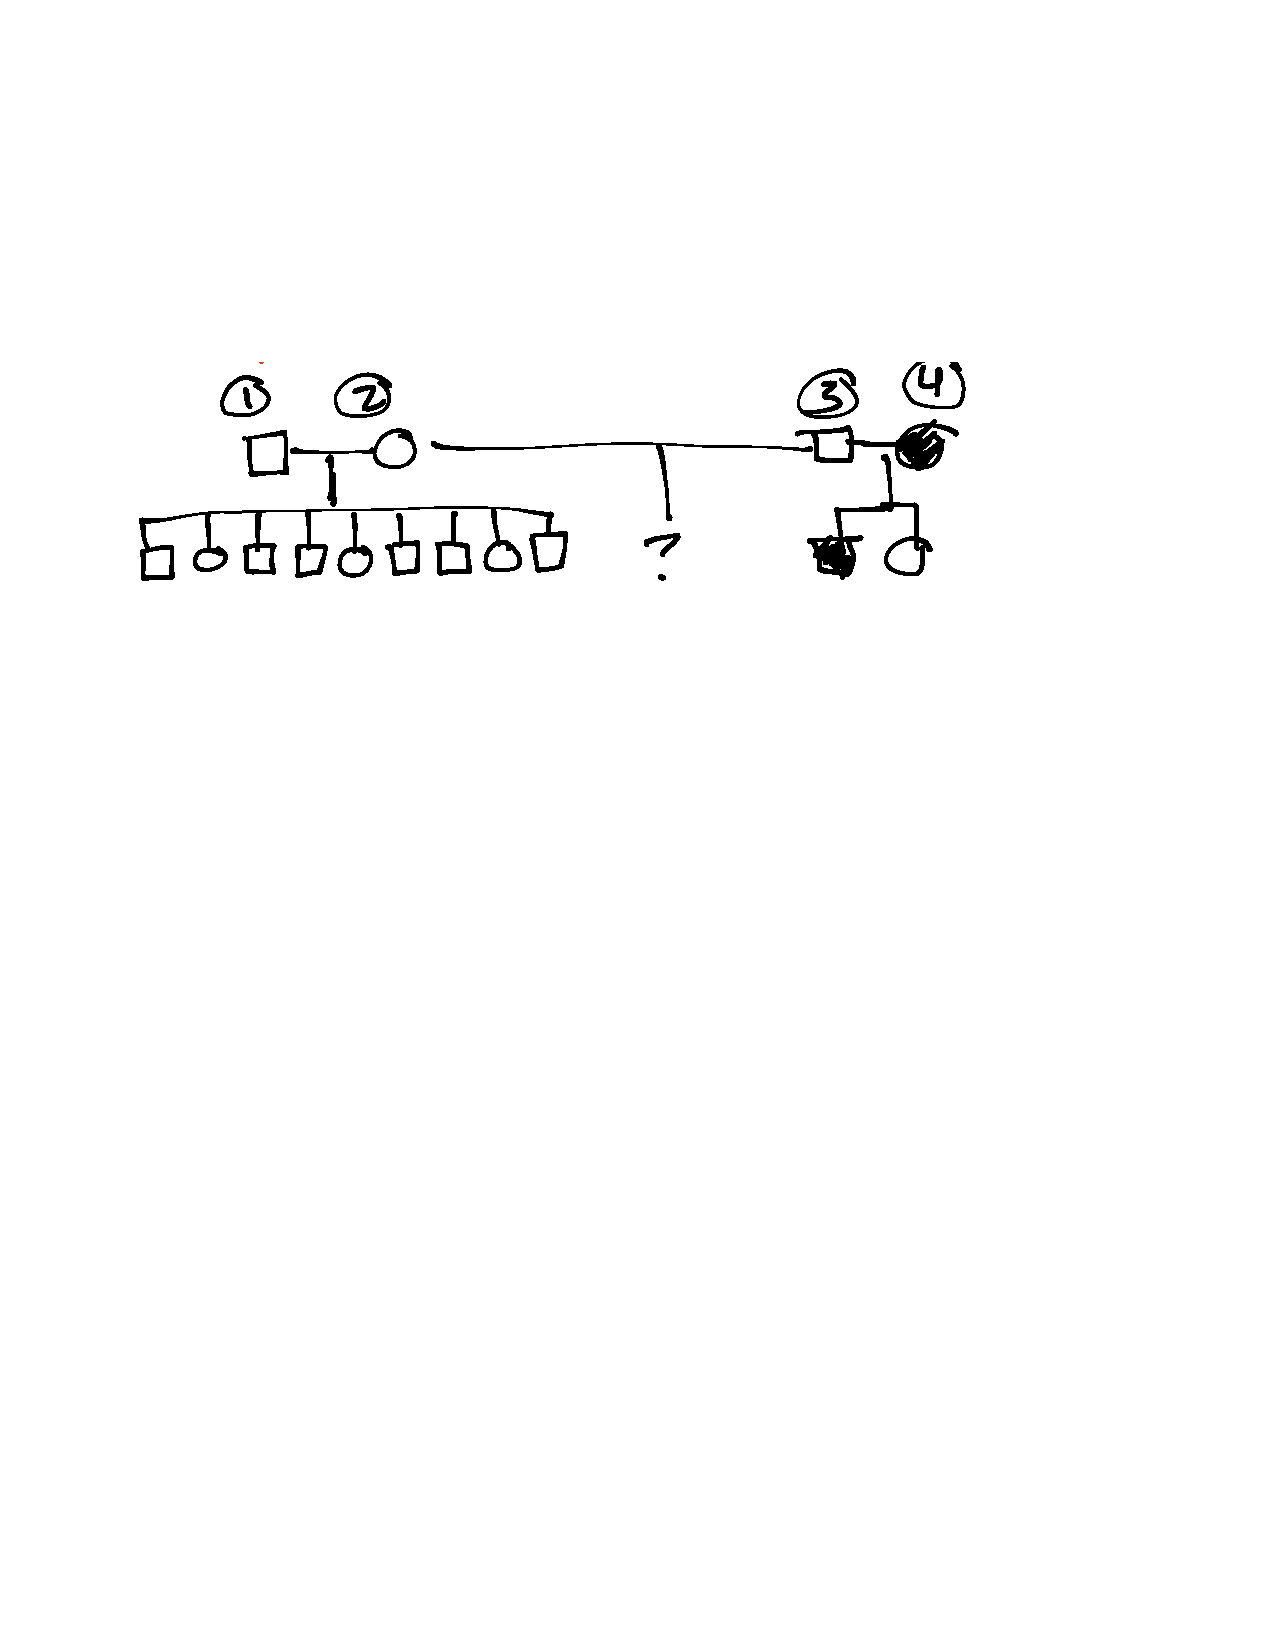
\includegraphics[width=130mm]{/Users/jri/src/bis101/images/pedigree_test.pdf}
\caption{A pedigree of miniature schnauzers. Filled symbols (square=male, circle=female) represent dogs with Von-Willibrands disease. Empty symbols are dogs with wild-type phenotypes.}
\label{dogigree}
  \end{center}
\end{figure*}
%-------------------------------------------------------------------

\newpage

\item You are interested in understanding the genetics of furriness in rabbits. You recruit 18 rabbit owners to bring in their bunnies for measurement.  Each bunny's fluffiness is measured on a scale of 1 (no hair) to 10 (maximum fluffy). Phenotypes for all 18 bunnies are shown in Table \ref{fluffy}. 

\begin{enumerate}
\item Calculate the phenotypic variance for fluffiness (5 pts).
\item In a separate study, you measure the fluffiness of a set of rabbit quadruplets that were sold by a breeder to 4 different families.  The phenotypic variance among these four genetically identical rabbits is 3.2. If we can assume that these families are representative of the environments of the rabbits in Table \ref{fluffy}, what is the broad sense heritability of fluffiness (5 pts).

%Their phenotypes are shown in Table \ref{clones}. Using these data, calculate the broad sense heritability of fluffiness in rabbits (6 pts).
\end{enumerate}

\begin{table}[h!]
\caption[]{Rabbit phenotypes.}
\begin{center}
\begin{tabular}{ll}
Rabbit Name & Fluffiness \\  \hline
Baby & 2\\
Baggins & 8\\
Bambi & 9\\
Barbie & 10\\
Basil & 7\\
Bella & 2\\
Benny & 7\\
Big Boy & 5\\
Big-Ears & 2\\
Binky & 10\\
Bluebell & 8\\
Boo Boo & 8\\
Buddy & 4\\
Bugs & 4\\
Bun Bun & 4\\
Bunnicula & 3\\
Bunzilla & 6\\
Buttercup & 4\\
\end{tabular}
\end{center}
\label{fluffy}
\end{table}

%\begin{table}[h!]
%\caption[]{Quadruplet rabbit phenotypes.}
%\begin{center}
%\begin{tabular}{ll}
%Rabbit Name & Fluffiness \\  \hline
%Oliver & 7\\
%Ollie & 8\\
%Oreo & 9\\
%Oscar & 9\\
%\end{tabular}
%\end{center}
%\label{clones}
%\end{table}

\newpage

\item Abscisic acid is an important regulator of seed maturation and germination in plants. You have two mutant maize plants that make insufficient levels of abscisic acid and thus their kernels germinate prematurely on the cob. When you self the first mutant it produces 345 mutant offspring. When you cross the second mutant to a wild-type plant all of the F1 are wild-type, and selfing the F1 results in 265 wild-type and 89 mutant offspring.  When you cross both original mutants together they produce 563 wild-type offspring.  Draw the genotypes of both mutant lines and the dominance of the alleles involved (10 pts).


%$A_1/A_2$ and $A_3/A_3$.  Two or three alleles at one locus ($A_2$ and $A_3$ could be same allele). $A_3$ is recessive. $A_1$ is dominant to $A_2$ and $A_3$
\newpage
\item The following two questions refer to the paper by Schempske and Bradshaw (1999). 
\begin{enumerate}
\item Briefly describe Schempske and Bradshaw's conclusions regarding the effect size of alleles important for speciation in \emph{Mimulus} (5pts).
%\item Provide an explanation for the different effects of the nectar QTL shown in Figure. 4A an 4B.
\item Carotenoid content in \emph{Mimulus} flowers is controlled by a single Mendelian locus called \emph{yup}. At this locus the \emph{M. cardinalis} allele is recessive to the \emph{M. lewissii} allele. In a population of F2 plants generated from a cross between \emph{M. lewissii}  and \emph{M. cardinalis}, provide an estimate and an explanation as to what you think the broad sense heritability for the orange/red color would be (\emph{hint: no calculations are needed to answer this question})(5 pts).
\end{enumerate}

%High (say above 60%) because single gene of large effect. Should be <100% because there will be environmental variation.
\newpage
\item Figure \ref{homologs} shows the karyotype of two individual plants of the genus\emph{Silene}.  The duplicated gene shown codes for an inorganic compound which causes plant tissue to appear significantly darker. The copy on chromosome 1 is expressed only in leaves, and the copy on chromosome 2 is expressed only in flower petals. Both loci are haplosufficient. (\emph{hint: reading Liu et al. 2012 may be helpful for figuring out this problem}).

\begin{enumerate}
\item Draw the karyotype and phenotype of the F1 and all possible F2 (6 pts).
\item I make a mutant version of I207 in the lab which has pale flowers and breeds true. Sequencing shows this mutant is homozygous for a mutation in the gene on chromosome 2 shown in figure \ref{homologs}. If I cross this mutant line with the F1 between wild-type I207 and B97, what proportion of the offspring will have pale flowers (4 pts)?

\end{enumerate}

\begin{figure*}[h!]
  \begin{center}
   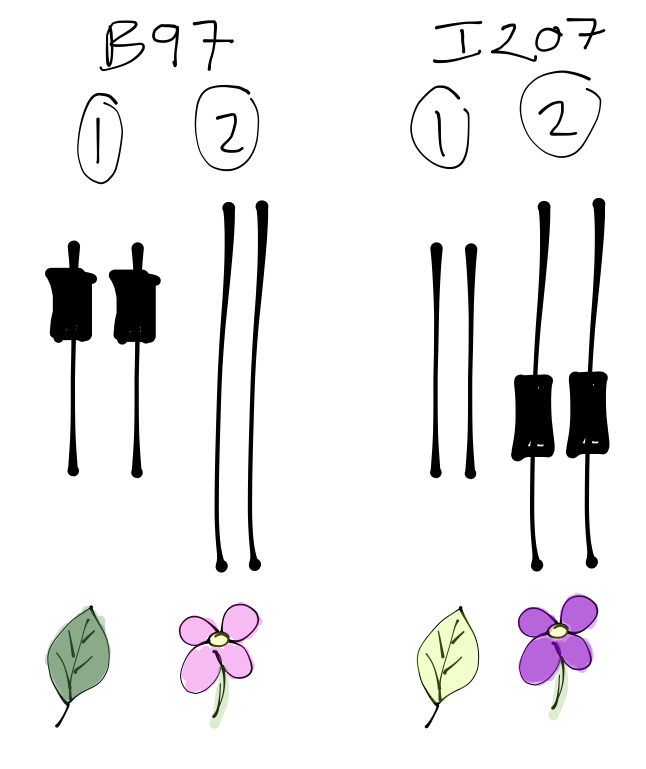
\includegraphics[width=80mm]{images/homologs.png}
    \caption{Karyotype for chromosomes 1 and 2 of \emph{Silene} lines B97 and I207. Boxes on each chromosome represent the presence of a gene of interest (the absence of a box signifies that the gene is not present on that chromosome). The flower and leaf phenotype of each line is shown below the karyotype: B97 has dark leaves and pale flowers and I207 has pale leaves and dark flowers.} 
\label{homologs}
  \end{center}
\end{figure*}

\newpage
\item Use the phylogeny of the gene \emph{ahbp3} shown in figure \ref{duplicates} to answer the following questions.

\begin{enumerate}
\item What term would you use to describe the relationship between the copies of \emph{ahbp3} in rice and \emph{Sorghum} marked in red in figure \ref{duplicates}  (2 pts)?
%paralogs
\item What evolutionary process would you ascribe to the gene copies in  \emph{Zea} marked in pink in figure \ref{duplicates} (2 pts)?
%subfunctionalization
\item Which of the gene copies in \emph{Zea} marked in blue in figure \ref{duplicates} is more likely to be in a syntenic position relative to \emph{Sorghum} (2 pts)?
%neofunctionalization
\item In what tissues do you think the gene copy ancestral to all the plants shown was expressed (2 pts)?
%roots and leaves
\item If you compare the sequence of the \emph{Zea }copy of \emph{ahbp3} expressed only in flowers to the \emph{ahbp3} locus in \emph{Agave}, what do you predict would be the relationship between nonsynonymous substitutions and synonymous substitutions, and why (2pts)?
%dn/ds >1 neofunctionalization


\end{enumerate}


\begin{figure*}[h!]
  \begin{center}
   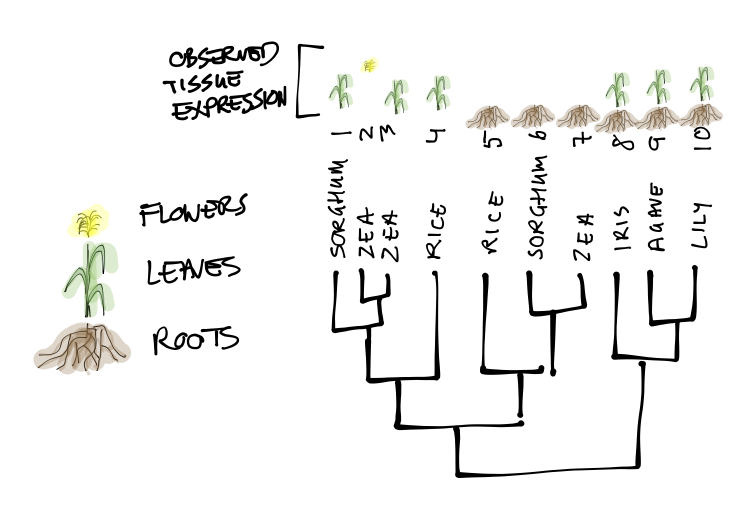
\includegraphics[width=110mm]{images/examfig2.png}
    \caption{Shown is a phylogenetic tree of the sequences of the \emph{ahbp3} locus in a groups of plants. The genus \emph{Zea} has 3 copies of this gene, while\emph{Sorghum} and rice each have two. Above the phylogeny is shown the tissues in which each copy is expressed. } 
\label{duplicates}
  \end{center}
\end{figure*}

\newpage

\item Johnston
\newpage
\item Genetic mapping
\newpage
\item Ibarra-Laclette 
\newpage
\item Chromosomal evolution
\end{enumerate}

\end{document}
